\documentclass{article}
\usepackage[utf8]{inputenc}
\usepackage[T1]{fontenc}
\usepackage{tikz, pgfplots}
\usetikzlibrary{angles}

\begin{document}

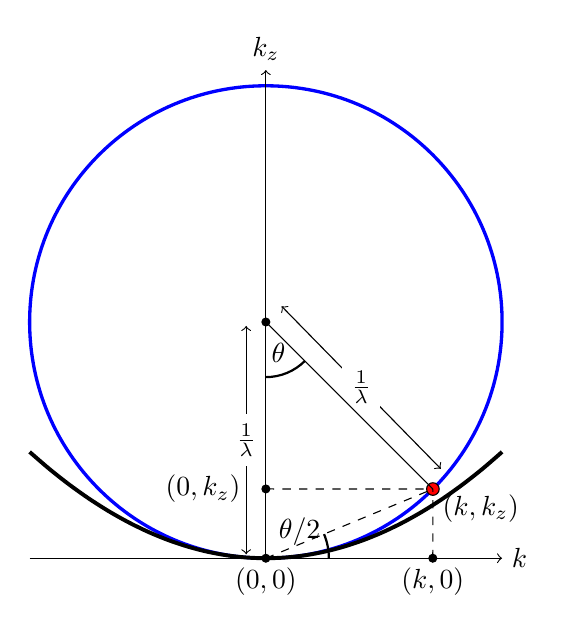
\begin{tikzpicture}
    %circle
    \draw[very thick, blue] (0,0) circle (3);

    %1/lambda
    \draw[<->] (-40:2.9) -- node[midway,fill=white] {$\frac{1}{\lambda}$} (0.2,0.2);
    \draw[<->] (-0.25,-0.05) -- node[midway,fill=white] {$\frac{1}{\lambda}$} (-0.25,-2.95);

    %axes
    \draw[->] (0,-3) -- (0,3.2) node[above] {$k_z$};
    \draw[->] (-3,-3) -- (3,-3) node[right] {$k$};

    %black points
    \draw[fill=black] (0,0) circle (0.05);
    \draw[fill=black] (0,-3) circle (0.05) node[below] {$(0,0)$};
    \draw[fill=red] (-45:3) circle (0.08) node[right, yshift=-0.25cm] {$(k,k_z)$};
    \draw[fill=black] (2.12,-3) circle (0.05) node[below] {$(k,0)$};
    \draw[fill=black] (0,-2.12) circle (0.05) node[left, xshift=-0.2cm] {$(0,k_z)$};

    %diagonal solid line joining black points
    \draw[](0,0) -- (-45:3);

    %dashed lines
    \draw[dashed] (2.12,-3) -- (-45:3);
    \draw[dashed] (0,-2.12) -- (-45:3);
    \draw[dashed](0,-3) -- (-45:3);

    %angles
    \draw (-45:3) coordinate (A)  (0,0) coordinate (B)
          (0,-3) coordinate (C)
           pic [draw,black,thick,angle radius=0.7cm, pic text=$\theta$] {angle = C--B--A};
    \draw (-45:3) coordinate (A)  (0,-3) coordinate (B)
          (3,-3) coordinate (C)
           pic [draw,black,thick,angle radius=0.8cm, angle eccentricity=1.5, pic text=$\theta/2$, pic text options={shift={(-0.75, 0.1)}}] {angle = C--B--A};

   %parabola
   \draw[black, line width = 0.50mm]   plot[smooth,domain=-3:3] (\x, {0.15*\x*\x-3});
\end{tikzpicture}

\end{document}